  Формы сигналов, которые получает монитор светимости имею размерность в единицах ацп на канал. Необходимо получать значения в энергитических единицах. Следовательно, стоит задача определения цены деления ацп для каждого канала. Для этой цели была разработана процедура энергетической калибровки онлайн монитора светимости. Процедура основывается на посылке тестового сигнала и сравнения амплитуд с монитора светимости и уже откалиброванной системой DAQ. Калибровочные коэффициенты расчитываются следующим образом:
\begin{equation}
  k = \frac{A_{DAQ}}{A_{LOM}}
\end{equation}
 где $A_{DAQ}$ и $A_{LOM}$ амплитуды с системы сбора данных DAQ и монитора светимости соответственно.\par
  Подробная схема данной процедуры представлена на рисунке 11 и заключается в следующем:
\begin{enumerate}
  \item На электромагнитный калориметр при помощи генератора импульсов, подается тестовый сигнал
  \item Далее сигнал проходит все системы до монитора светимости как реальный сигнал
  \item На выходе с монитора светимости получаем амплитудные значения в каналах АЦП
  \item Далее вычисляются калибровочные коэффициенты по формулеХ
\end{enumerate}\par
\begin{figure}[htp]
  \centering
  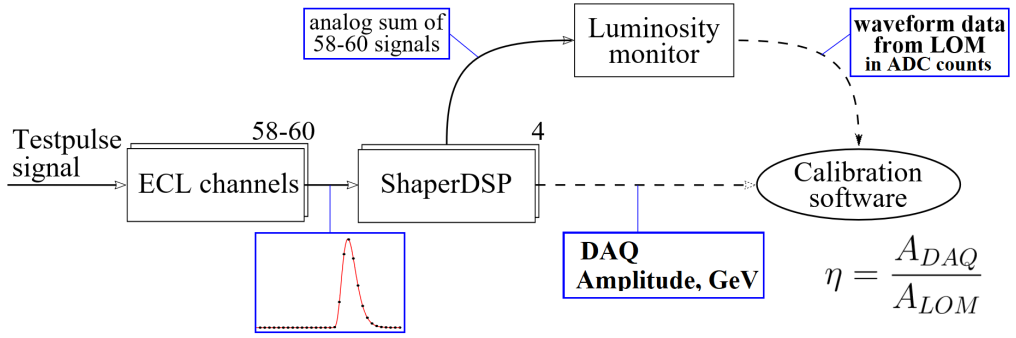
\includegraphics[width=\textwidth]{calibration.png}
  \caption{Процесс энергетической калибровки монитора светимости}
  \label{fig:galaxy}
\end{figure}
  Так как в процессе энергетической калибровки необходимо параллельно читать данные с монитора светимости и амплитудные значения с системы сбора данных DAQ, то нужно иметь возможность управлять чтением данных с монитора светимости. Требуется останавливать и продолжать чтение данных в любой момент времени. Для реализации данной возможности был расширен протокол монитора светимости. Были добавлены команды, которые позволяют остановить чтение данных с монитора светимости, возобновить чтение данных и посмотреть текущий статус монитора светимости.\par
  Также для автоматизации контроля актуальной версии калибровочных коээфициентов, было реализовано хранение калибровочных коэффициентов в базе данных DAQ. При запуске ПО  проверяется ищет последнюю версию калибровочных коэффициентов и используется в дальнейшем.\par
  В торцах электромагнитного калориметра находится 2112 кристаллов, однако монитор светимости в конечном итоге получает суммированную информацию с этих каналов, сгруппированную по 32 секторам. Таким образом форма сигнала для каждого сектора -- это сумма форм сигналов от, в среднем, 2112/32 = 66 каналов. Однако, все кристаллы обладают немного разными физическими характеристиками, в частности, разным световыходом (light yield), требуется суммировать сигналы с неким весом. Этот вес называется коэффициент аттенюации. Проанализировав изменения аттенюаторных и калибровочных коэффициенто, было замечено, что они коррелирует друг с другом. Поэтому для более детального анализа, сравнили изменения аттенюаторных коээфициентов и калибровочных за одинаковые промежутки времени. Результат сравнения представлен на рисунке 12. Таким образом можно проверять если изменинлись аттенюаторные коэффициенты, то на соответствующую величину изменять и калибровочные коэффициенты.
\newpage
\begin{figure}[htp]
  \centering
  \includegraphics[width=\textwidth]{coefs_new.pdf}
  \caption{Изменение калибровочных и аттенюаторных коэффициентов за равный промежуток времени}
  \label{fig:galaxy}
\end{figure}
